\documentclass[11pt,a4paper]{article}

\usepackage[utf8]{inputenc}
\usepackage[T1]{fontenc}
\usepackage[margin=2.3cm]{geometry}
\usepackage{xcolor}
\usepackage{hyperref}
\usepackage{booktabs}
\usepackage{longtable}
\usepackage{array}
\usepackage{enumitem}
\usepackage{amsmath,amssymb}
\usepackage{tikz}
\usetikzlibrary{arrows.meta,positioning,fit,backgrounds,shapes.geometric}
\usepackage{tcolorbox}
\tcbuselibrary{skins,breakable}
\usepackage{fancyhdr}

\definecolor{primary}{RGB}{31,73,125}
\definecolor{teal}{RGB}{0,128,128}
\definecolor{red}{RGB}{178,34,34}
\definecolor{green}{RGB}{46,125,50}
\definecolor{gray}{RGB}{242,242,242}

\hypersetup{colorlinks=true,linkcolor=primary,urlcolor=teal,
  pdftitle={AI Integration Guide for the Autonomous Earthen Heritage UAV}}
\pagestyle{fancy}
\fancyhf{}
\fancyhead[L]{\small Autonomous Earthen Heritage UAV}
\fancyhead[R]{\small AI Integration Guide}
\fancyfoot[C]{\thepage}
\newcommand{\code}[1]{\texttt{\small #1}}
\newtcolorbox{important}[1]{enhanced,breakable,colback=gray,colframe=primary,
  title=#1,fonttitle=\bfseries}
\newtcolorbox{warning}[1]{enhanced,breakable,colback=red!5,colframe=red,
  title=#1,fonttitle=\bfseries}
\newtcolorbox{acceptance}[1]{enhanced,breakable,colback=green!6,colframe=green,
  title=#1,fonttitle=\bfseries}

\title{\color{primary}\Huge\bfseries
  AI Integration Guide\\[0.25em]
  \Large RAG-VLM and YOLOv11 on the Validated PX4/Gazebo Simulation}
\author{UAS Infrastructure Monitoring Team}
\date{Integration reference --- August 2026}

\begin{document}
\maketitle
\thispagestyle{empty}

\begin{important}{Purpose of this document}
This document explains how the Person 1 AI branch must be integrated with the
validated simulation on \code{main}. It is not a request to replace the
Gazebo/PX4/MAVROS stack. The simulation, camera bridge, rosbag recorder,
waypoint trigger, and A* planner are the platform contract. RAG-VLM, raw VLM,
and YOLOv11 are interchangeable detector implementations layered on top of
that contract.
\end{important}

\tableofcontents
\newpage

\section{Project End Goal}

The project is a comparative empirical study for autonomous inspection of
earthen heritage architecture. The contribution is not a new VLM, detector,
or path planner. The study compares three detector paradigms and two
inspection strategies:

\begin{center}
\begin{tabular}{lll}
\toprule
Condition & Detector & Strategy \\
\midrule
C1 & Raw zero-shot VLM & Single pass \\
C2 & Raw zero-shot VLM & Confidence-triggered revisit \\
C3 & RAG-grounded VLM & Single pass \\
C4 & RAG-grounded VLM & Confidence-triggered revisit \\
C5 & Trained YOLOv11 & Single pass \\
C6 & Trained YOLOv11 & Confidence-triggered revisit \\
\bottomrule
\end{tabular}
\end{center}

The blueprint requires post-flight, waypoint-decoupled inference. The vehicle
records the camera continuously, but AI inference runs on one frame captured
per inspection waypoint. This prevents a VLM from trying to process a 30 FPS
stream and preserves a fair comparison between detectors.

\section{Validated Simulation Architecture}

The current simulation is a working PX4 SITL/Gazebo Harmonic system. It must
remain independent of the AI model selected for a particular experiment.

\begin{center}
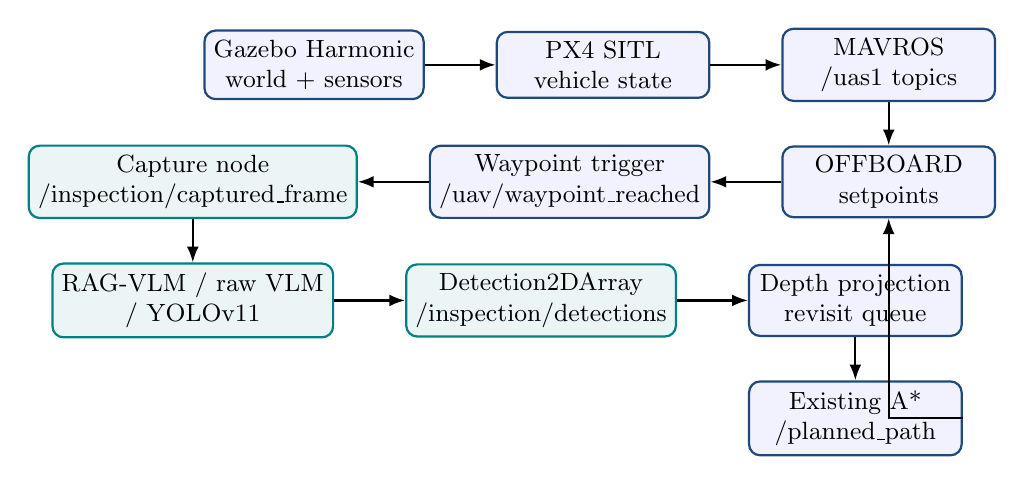
\begin{tikzpicture}[
  node distance=0.55cm and 0.9cm,
  box/.style={draw=primary, thick, rounded corners, fill=blue!5,
    minimum width=2.7cm, minimum height=0.8cm, align=center, font=\small},
  ai/.style={draw=teal, thick, rounded corners, fill=teal!8,
    minimum width=2.7cm, minimum height=0.8cm, align=center, font=\small},
  arrow/.style={-{Latex[length=2mm]}, thick}
]
\node[box] (gz) {Gazebo Harmonic\\world + sensors};
\node[box, right=of gz] (px4) {PX4 SITL\\vehicle state};
\node[box, right=of px4] (mavros) {MAVROS\\/uas1 topics};
\node[box, below=of mavros] (setpoint) {OFFBOARD\\setpoints};
\node[box, left=of setpoint] (trigger) {Waypoint trigger\\/uav/waypoint\_reached};
\node[ai, left=of trigger] (capture) {Capture node\\/inspection/captured\_frame};
\node[ai, below=of capture] (detector) {RAG-VLM / raw VLM\\/ YOLOv11};
\node[ai, right=of detector] (detections) {Detection2DArray\\/inspection/detections};
\node[box, right=of detections] (revisit) {Depth projection\\revisit queue};
\node[box, below=of revisit] (astar) {Existing A*\\/planned\_path};

\draw[arrow] (gz) -- (px4);
\draw[arrow] (px4) -- (mavros);
\draw[arrow] (mavros) -- (setpoint);
\draw[arrow] (setpoint) -- (trigger);
\draw[arrow] (trigger) -- (capture);
\draw[arrow] (capture) -- (detector);
\draw[arrow] (detector) -- (detections);
\draw[arrow] (detections) -- (revisit);
\draw[arrow] (revisit) -- (astar);
\draw[arrow] (astar) -| (setpoint);
\end{tikzpicture}
\end{center}

\subsection{Stable topic contract}

\begin{longtable}{p{0.38\linewidth}p{0.52\linewidth}}
\toprule
\textbf{Topic} & \textbf{Role} \\
\midrule
\code{/camera/color/image\_raw} & Canonical live RGB stream from the discovered Gazebo bridge. \\
\code{/camera/color/camera\_info} & Camera intrinsics for downstream geometry. \\
\code{/camera/depth/image\_raw} & Canonical depth stream when \code{gz\_x500\_depth} is selected. \\
\code{/uas1/local\_position/pose} & MAVROS local vehicle pose. \\
\code{/uas1/setpoint\_position/local} & MAVROS setpoint stream used by the waypoint adapter. \\
\code{/uav/waypoint\_reached} & Integer trigger emitted when a setpoint is reached. \\
\code{/inspection/captured\_frame} & One RGB frame forwarded to the selected detector. \\
\code{/inspection/detections} & \code{vision\_msgs/msg/Detection2DArray} output. \\
\code{/planner/revisit\_waypoints} & PoseArray input consumed by the existing planner. \\
\code{/planned\_path} & Path output consumed by the current path follower. \\
\bottomrule
\end{longtable}

The raw Gazebo names are model-dependent. They must not be used as the AI
interface. The bridge maps them to the canonical ROS names above.

\section{What the Person 1 Branch Does Now}

The branch \code{feature/person1-ai-vlm-rag} adds a Qwen2.5-VL-3B-Instruct
detector, a HuggingFace CLIP knowledge-base retriever, an offline embedding
builder, and standalone model demonstrations. Those are useful building
blocks, but the branch is based on the pre-camera-fix project state.

The current branch has the following integration problems:

\begin{enumerate}[leftmargin=1.2cm]
\item \textbf{Capture plumbing is removed.} The branch removes
\code{waypoint\_reached\_node.py} from the launch file, CMake installation,
and Python entry points. No waypoint trigger means no captured frames.
\item \textbf{The package does not build.} \code{setup.py} contains
\code{zip\_safe=true}; Python requires \code{zip\_safe=True}.
\item \textbf{AI dependencies are not installed in the active image.} The
current simulation container has ROS2, PX4, Gazebo, PyTorch CPU, and YOLO, but
not Transformers, BitsAndBytes, or Accelerate.
\item \textbf{Relative model paths are unsafe in Docker.} Paths must resolve
through \code{UAS\_INSPECTION\_ROOT=/home/uas/inspection}.
\item \textbf{RAG is initialized for every backend.} YOLO must not load CLIP
or Qwen dependencies when the selected backend is \code{yolo}.
\item \textbf{Random fallback output is not research output.} Missing models,
embeddings, or invalid VLM text must produce an explicit failure or an
explicitly labelled mock result, never a plausible random detection.
\item \textbf{The branch changes the pose topic to \code{/px4/vehicle\_pose},}
which is not published by the current MAVROS setup.
\end{enumerate}

\begin{warning}{Integration rule}
Port the AI implementation into \code{main}; do not merge the branch as a
replacement tree. Preserve the current launch, camera, rosbag, waypoint,
MAVROS, and navigation files.
\end{warning}

\section{Correct VLM Integration}

\subsection{Detector lifecycle}

The detector node must subscribe to \code{/inspection/captured\_frame}, not
the 30 FPS RGB topic. Its callback should:

\begin{enumerate}[leftmargin=1.2cm]
\item Convert the ROS image using \code{cv\_bridge}.
\item Retrieve top-$k$ context only for \code{rag\_vlm}.
\item Construct the raw or grounded prompt.
\item Run Qwen inference on the single captured frame.
\item Parse a strict structured response.
\item Normalize the class to an ontology ID.
\item Clamp and validate the bounding box.
\item Publish \code{Detection2DArray} with the original image header.
\item Record latency, backend, model version, prompt version, and result.
\end{enumerate}

For a CPU-only machine, Qwen inference must be treated as offline/batch
processing. It must not be allowed to block flight control or the camera
bridge. A separate AI container or offline rosbag replay is preferred.

\subsection{Backend separation}

The node must instantiate only one backend:

\begin{verbatim}
raw_vlm -> Qwen model, generic prompt, no CLIP retrieval
rag_vlm -> CLIP retriever + Qwen model + grounded prompt
yolo    -> Ultralytics YOLO model only
\end{verbatim}

All three backends must implement the same method:

\begin{verbatim}
detect(image_bgr) -> [
  {"bbox": [xmin, ymin, xmax, ymax],
   "class_id": "structural_crack",
   "confidence": 0.0..1.0}
]
\end{verbatim}

The ROS adapter must publish the same message type regardless of backend.

\subsection{RAG knowledge base}

The blueprint calls for 20--40 curated entries and 3--5 reference crops per
class. The current repository contains an ontology skeleton and placeholder
crop directories; it is not yet a complete research knowledge base.

Each entry should contain:

\begin{verbatim}
id: structural_crack
name: Structural Crack
description: concise domain description
prompt_template: VLM grounding text
ref_crops: [absolute or project-resolved image paths]
\end{verbatim}

The offline builder must:

\begin{enumerate}[leftmargin=1.2cm]
\item Load the ontology and verify every crop exists.
\item Fail if Transformers/CLIP is unavailable unless \code{--mock} is used.
\item Encode text descriptions and reference crops with the same CLIP model.
\item Normalize and combine embeddings deterministically.
\item Save the embedding index with model ID, embedding dimension, ontology
version, and creation timestamp.
\end{enumerate}

At runtime, the retriever should fail clearly if the cache is absent or has an

\subsection{Structured VLM output}

The prompt should request JSON rather than a permissive regex string:

\begin{verbatim}
{
  "detections": [
    {"class_id": "structural_crack",
     "bbox_xyxy": [xmin, ymin, xmax, ymax],
     "confidence": 0.0}
  ]
}
\end{verbatim}

The parser must reject malformed output, reject unknown classes, normalize

\section{YOLOv11 Integration}

YOLOv11 is not a separate demonstration. It is the supervised baseline in the

\subsection{Training pipeline}

The training data must combine SDNET2018, MBDD2025, and earthen-domain

From the repository root, the current training entry point is:

\begin{verbatim}
python3 scripts/train_yolov11.py \\
  --data-yaml data/earthen_defects.yaml \\
  --epochs 50 \\
  --batch-size 16 \\
  --output models/yolo/yolo_earthen_v11.pt
\end{verbatim}

The script uses \code{yolo11s.pt}, writes the Ultralytics run under

\subsection{ROS2 YOLO backend}

The YOLO backend must:

\begin{enumerate}[leftmargin=1.2cm]
\item Load only \code{models/yolo/yolo\_earthen\_v11.pt}.
\item Process \code{/inspection/captured\_frame} by default.
\item Publish \code{Detection2DArray} exactly like the VLM backends.
\item Convert every class index to a canonical ontology ID.
\item Preserve confidence values without replacing them with constants.
\item Log model path, image size, inference device, and latency.
\item Return an empty list when no detection is produced.
\end{enumerate}

A missing weights file must be a visible configuration error. A mock YOLO

\subsection{YOLO and revisit strategy}

YOLO single-pass and YOLO revisit must use the same code path as VLM:

\begin{verbatim}
waypoint trigger
  -> captured RGB frame
  -> YOLO detection
  -> confidence filtering
  -> optional depth projection
  -> revisit PoseArray
  -> existing A* planner
  -> second captured frame
  -> YOLO detection again
\end{verbatim}

No YOLO-specific planner or topic is required.

\section{Revisit and Coordinate Requirements}

The current revisit generator computes pinhole coordinates:

\begin{equation}
X = \frac{(u-c_x)Z}{f_x}, \qquad
Y = \frac{(v-c_y)Z}{f_y}, \qquad
Z = D(u,v).
\end{equation}

Those coordinates are in the camera optical frame. They must not be published

\begin{enumerate}[leftmargin=1.2cm]
\item transform the point through TF2 using the camera pose and vehicle pose;
or
\item explicitly define a simulation-only fixed camera-to-map transform and
\end{enumerate}

The revisit node should queue all ambiguous detections from the primary pass,

\section{Environment and Container Strategy}

The PX4/Gazebo simulation container is already responsible for heavy robotics

Preferred arrangement:

\begin{enumerate}[leftmargin=1.2cm]
\item Keep \code{uas\_sim} responsible for PX4, Gazebo, MAVROS, camera bridge,
\item Build a separate AI/VLM image with Transformers, CLIP, Qwen, and
\item Run real VLM inference on captured frames or rosbag replay.
\item Keep YOLO available in the AI image and optionally in \code{uas\_sim}
\item Never make camera recording or flight control depend on a model download.
\end{enumerate}

The Qwen model card recommends a current Transformers build because older

\section{Commands for the Integration Test}

Start the validated simulation first:

\begin{verbatim}
cd Autonomous-Drone-Inspection
xhost +local:
docker compose --project-directory . -f docker/docker-compose.yml \\
  --profile sim build sim_stack
docker compose --project-directory . -f docker/docker-compose.yml \\
  --profile sim up -d --force-recreate sim_stack
docker exec -it uas_sim bash -lc '/home/uas/docker/bootstrap_px4.sh'
docker exec uas_sim bash -lc '/home/uas/scripts/build_workspace.sh'
./docker/launch_obstacle_stack.sh --gui
\end{verbatim}

Verify the camera and ROS contracts:

\begin{verbatim}
docker exec uas_sim bash -lc 'source /opt/ros/humble/setup.bash; \\
  ros2 topic hz /camera/color/image_raw'
docker exec uas_sim bash -lc 'source /opt/ros/humble/setup.bash; \\
  ros2 topic list | grep -E "uav|inspection|camera|uas1"'
\end{verbatim}

After a flight, export the canonical RGB video and telemetry:

\begin{verbatim}
docker exec uas_sim bash -lc 'source /opt/ros/humble/setup.bash; \\
  python3 /home/uas/scripts/analysis/analyze_rosbags.py \\
  --bag latest --export-csv --export-video \\
  --video-topic /camera/color/image_raw'
\end{verbatim}

Launch the inspection package only after building the workspace and only after
the capture trigger has been preserved:

\begin{verbatim}
docker exec uas_sim bash -lc 'source /opt/ros/humble/setup.bash; \\
  source /home/uas/ros2_ws/install/setup.bash; \\
  ros2 launch uas_earthen_inspection inspection_pipeline.launch.py \\
  detector_backend:=yolo flight_strategy:=single_pass'
\end{verbatim}

\section{Acceptance Checklist}

\begin{acceptance}{Do not call the integration complete until all items pass}
\begin{enumerate}[leftmargin=1.2cm]
\item The simulation launches without AI dependencies installed.
\item \code{/camera/color/image\_raw} publishes live frames.
\item The rosbag contains nonzero canonical RGB samples.
\item \code{/uav/waypoint\_reached} is published when setpoints are reached.
\item \code{/inspection/captured\_frame} contains one frame per waypoint.
\item Each backend publishes valid \code{Detection2DArray} messages.
\item Missing models fail explicitly instead of producing research-looking
\item YOLO, raw VLM, and RAG-VLM can be selected without initializing the
\item Revisit points are transformed into the correct map frame.
\item A real, labelled evaluation set is used before reporting metrics.
\item C1--C6 logs contain measured precision, recall, latency, confidence
\end{enumerate}
\end{acceptance}

\section{Summary}

The teammate branch should be treated as a source of Qwen/CLIP implementation
ideas, not as a replacement for the simulation branch. The correct integration
preserves the validated ROS contracts, adds one detector backend at a time,

\end{document}
